\documentclass[aspectratio=169,10pt]{beamer}
\usepackage[utf8]{inputenc}
\usepackage[T1]{fontenc}
\usepackage{amsmath,amsfonts,amssymb}
\usepackage{graphicx}
\usepackage{xcolor}
\usepackage{tikz}
\usetikzlibrary{shapes,arrows.meta,positioning,fit,calc,shadows,decorations.pathreplacing}
\usepackage{booktabs}
\usepackage{array}
\usepackage{colortbl}
\usepackage{listings}
\usepackage{hyperref}

\usetheme{Madrid}
\usecolortheme{default}
\setbeamertemplate{navigation symbols}{}
\setbeamertemplate{footline}[frame number]

\AtBeginSection[]{}
\AtBeginSubsection[]{}

\definecolor{mlblue}{RGB}{0,102,204}
\definecolor{mlgreen}{RGB}{0,153,76}
\definecolor{mlorange}{RGB}{255,102,0}
\definecolor{mlred}{RGB}{204,0,51}
\definecolor{mlpurple}{RGB}{102,51,153}
\definecolor{codebg}{RGB}{245,245,248}

\setbeamercolor{structure}{fg=mlblue}
\setbeamercolor{block title}{bg=mlblue,fg=white}
\setbeamercolor{block body}{bg=mlblue!8}
\setbeamercolor{alerted text}{fg=mlred}
\setbeamercolor{example text}{fg=mlgreen}

\lstdefinestyle{pythonstyle}{
    language=Python,
    basicstyle=\ttfamily\scriptsize,
    keywordstyle=\color{mlblue}\bfseries,
    commentstyle=\color{mlgreen!70!black}\itshape,
    stringstyle=\color{mlred},
    showstringspaces=false,
    breaklines=true,
    frame=single,
    rulecolor=\color{gray!40},
    backgroundcolor=\color{codebg},
    numbers=left,
    numberstyle=\tiny\color{gray},
    numbersep=4pt,
    xleftmargin=1.2em
}
\lstset{style=pythonstyle}

\title[API Design]{From Model to Medium}
\subtitle{Topic 2: API Design Principles}
\author{ML + UI + API + MCP Project}
\institute{Learning Path}
\date{\today}

\begin{document}

\begin{frame}
\titlepage
\end{frame}

\begin{frame}{Outline}
\tableofcontents
\end{frame}

\section{Why design matters}

\begin{frame}{An API is a contract}
\begin{columns}[T]
\begin{column}{0.48\textwidth}
\begin{block}{Key idea}
A well-designed API is predictable: a developer (or an AI assistant) can guess how it works before reading the docs.
\end{block}
\begin{itemize}
\item Clear endpoint names
\item Consistent request and response shapes
\item Helpful, uniform errors
\item Stable over time (versioning)
\end{itemize}
\end{column}
\begin{column}{0.48\textwidth}
\begin{center}
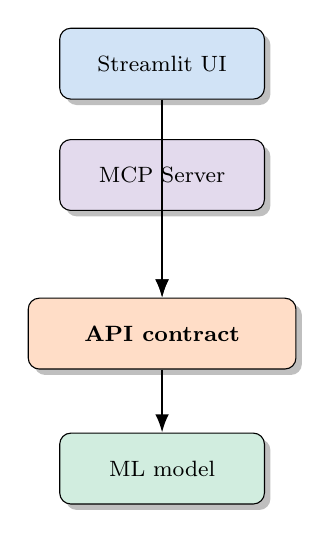
\begin{tikzpicture}[
  box/.style={draw, rounded corners, align=center, minimum height=0.9cm,
              minimum width=2.6cm, font=\footnotesize, drop shadow},
  arr/.style={-{Latex}, thick}
]
  \node[box, fill=mlblue!18] (ui) {Streamlit UI};
  \node[box, fill=mlpurple!18, below=0.5cm of ui] (mcp) {MCP Server};
  \node[box, fill=mlorange!22, below=1.1cm of mcp, minimum width=3.4cm] (api) {\textbf{API contract}};
  \node[box, fill=mlgreen!18, below=0.8cm of api] (ml) {ML model};
  \draw[arr] (ui) -- (api);
  \draw[arr] (mcp) -- (api);
  \draw[arr] (api) -- (ml);
\end{tikzpicture}
\end{center}
\end{column}
\end{columns}
\end{frame}

\section{Endpoints and URLs}

\begin{frame}{Anatomy of a URL}
\begin{center}
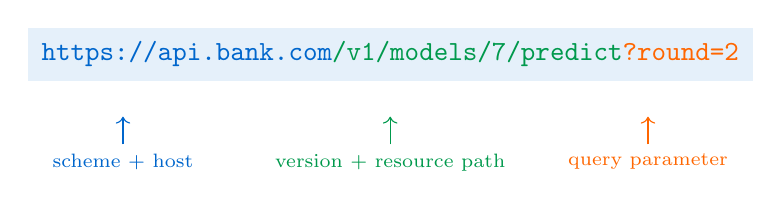
\begin{tikzpicture}[font=\small, lbl/.style={font=\scriptsize, align=center}]
  \node[font=\ttfamily\normalsize, fill=mlblue!10, inner sep=5pt] (url)
    {\textcolor{mlblue}{https://api.bank.com}\textcolor{mlgreen}{/v1/models/7/predict}\textcolor{mlorange}{?round=2}};
  \node[lbl, mlblue,   below left=0.8cm and -0.2cm of url.south west, anchor=north west] (l1) {scheme + host};
  \node[lbl, mlgreen,  below=0.8cm of url] (l2) {version + resource path};
  \node[lbl, mlorange, below right=0.8cm and -0.2cm of url.south east, anchor=north east] (l3) {query parameter};
  \draw[->, mlblue]   (l1.north) -- ++(0,0.35);
  \draw[->, mlgreen]  (l2.north) -- ++(0,0.35);
  \draw[->, mlorange] (l3.north) -- ++(0,0.35);
\end{tikzpicture}
\end{center}
\begin{block}{Rule}
The path identifies the \textbf{resource}; query parameters \textbf{filter or tweak} the result.
\end{block}
\end{frame}

\begin{frame}{Resource naming: nouns, not verbs}
\begin{columns}[T]
\begin{column}{0.48\textwidth}
\begin{alertblock}{Avoid (verbs)}
\texttt{/getAllModels}\\
\texttt{/createPrediction}\\
\texttt{/deleteModel?id=7}
\end{alertblock}
\end{column}
\begin{column}{0.48\textwidth}
\begin{exampleblock}{Prefer (nouns + method)}
\texttt{GET /models}\\
\texttt{POST /predictions}\\
\texttt{DELETE /models/7}
\end{exampleblock}
\end{column}
\end{columns}
\vspace{0.3cm}
\begin{itemize}
\item Use \textbf{plural} nouns and \texttt{lowercase-with-hyphens}.
\item The HTTP method already says the action.
\item Nest only when ownership is clear: \texttt{/models/7/predictions}.
\end{itemize}
\end{frame}

\begin{frame}{Resource tree of our ML API}
\begin{center}
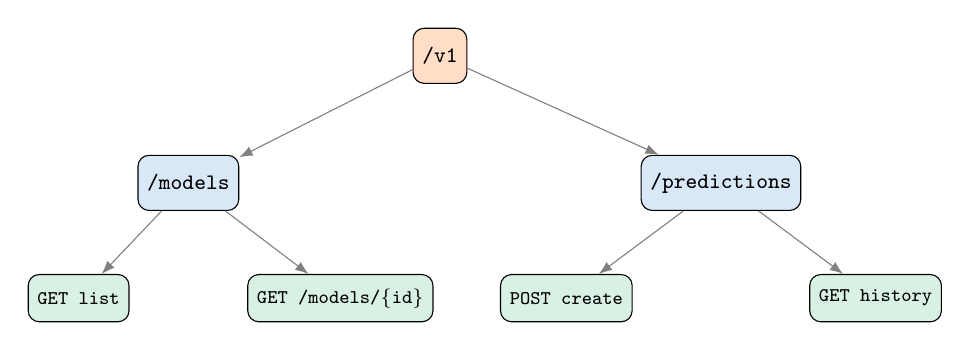
\begin{tikzpicture}[
  node distance=0.6cm and 0.5cm,
  res/.style={draw, rounded corners, fill=mlblue!15, font=\footnotesize\ttfamily, minimum height=0.7cm, align=center},
  act/.style={draw, rounded corners, fill=mlgreen!15, font=\scriptsize\ttfamily, minimum height=0.6cm, align=center},
  arr/.style={-{Latex}, gray}
]
  \node[res, fill=mlorange!22] (root) {/v1};
  \node[res, below left=0.9cm and 2.2cm of root] (models) {/models};
  \node[res, below right=0.9cm and 2.2cm of root] (preds) {/predictions};
  \node[act, below left=0.8cm and 0.1cm of models] (m1) {GET list};
  \node[act, below right=0.8cm and 0.1cm of models] (m2) {GET /models/\{id\}};
  \node[act, below left=0.8cm and 0.1cm of preds] (p1) {POST create};
  \node[act, below right=0.8cm and 0.1cm of preds] (p2) {GET history};
  \draw[arr] (root) -- (models);
  \draw[arr] (root) -- (preds);
  \draw[arr] (models) -- (m1);
  \draw[arr] (models) -- (m2);
  \draw[arr] (preds) -- (p1);
  \draw[arr] (preds) -- (p2);
\end{tikzpicture}
\end{center}
\end{frame}

\begin{frame}[fragile]{Easy sample: endpoints in FastAPI}
\begin{lstlisting}
from fastapi import FastAPI

app = FastAPI(title="House Price API")

@app.get("/v1/models")                  # list resources
def list_models():
    return [{"id": 1, "name": "linear_regression"}]

@app.get("/v1/models/{model_id}")       # one resource
def get_model(model_id: int):
    return {"id": model_id, "name": "linear_regression"}

@app.post("/v1/predictions")            # create a prediction
def create_prediction(features: dict):
    return {"predicted_price": 412500.0}
\end{lstlisting}
\end{frame}

\section{Schemas and Errors}

\begin{frame}[fragile]{Consistent request/response schemas}
\begin{columns}[T]
\begin{column}{0.52\textwidth}
\begin{lstlisting}
from pydantic import BaseModel

class PredictionRequest(BaseModel):
    square_feet: float
    bedrooms: int

class PredictionResponse(BaseModel):
    predicted_price: float
    model_version: str
\end{lstlisting}
\end{column}
\begin{column}{0.44\textwidth}
\begin{lstlisting}[numbers=none]
{
  "predicted_price": 412500.0,
  "model_version": "1.0.0"
}
\end{lstlisting}
\vspace{0.2cm}
\begin{block}{Tip}
Same field names and types everywhere: \texttt{snake\_case}, numbers as numbers.
\end{block}
\end{column}
\end{columns}
\end{frame}

\begin{frame}{Choosing the right status code}
\begin{center}
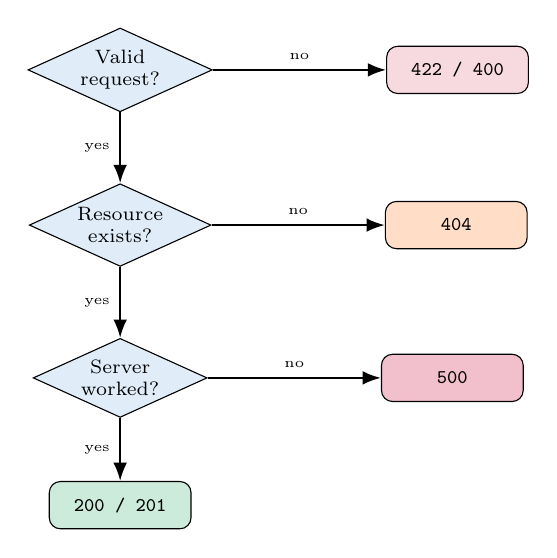
\begin{tikzpicture}[
  q/.style={draw, diamond, aspect=2.2, fill=mlblue!12, font=\scriptsize, align=center, inner sep=1pt},
  r/.style={draw, rounded corners, font=\scriptsize\ttfamily, minimum height=0.6cm, minimum width=1.8cm},
  arr/.style={-{Latex}, thick}
]
  \node[q] (q1) {Valid\\request?};
  \node[r, fill=mlred!15, right=2.2cm of q1] (e422) {422 / 400};
  \node[q, below=0.9cm of q1] (q2) {Resource\\exists?};
  \node[r, fill=mlorange!22, right=2.2cm of q2] (e404) {404};
  \node[q, below=0.9cm of q2] (q3) {Server\\worked?};
  \node[r, fill=mlred!25, right=2.2cm of q3] (e500) {500};
  \node[r, fill=mlgreen!20, below=0.8cm of q3] (ok) {200 / 201};
  \draw[arr] (q1) -- node[above, font=\tiny] {no} (e422);
  \draw[arr] (q1) -- node[left, font=\tiny] {yes} (q2);
  \draw[arr] (q2) -- node[above, font=\tiny] {no} (e404);
  \draw[arr] (q2) -- node[left, font=\tiny] {yes} (q3);
  \draw[arr] (q3) -- node[above, font=\tiny] {no} (e500);
  \draw[arr] (q3) -- node[left, font=\tiny] {yes} (ok);
\end{tikzpicture}
\end{center}
\end{frame}

\begin{frame}[fragile]{Predictable error handling}
\begin{lstlisting}
from fastapi import FastAPI, HTTPException

app = FastAPI()
MODELS = {1: "linear_regression"}

@app.get("/v1/models/{model_id}")
def get_model(model_id: int):
    if model_id not in MODELS:
        raise HTTPException(
            status_code=404,
            detail={"code": "MODEL_NOT_FOUND",
                    "message": f"Model {model_id} does not exist"},
        )
    return {"id": model_id, "name": MODELS[model_id]}
\end{lstlisting}
\begin{alertblock}{Rule}
Every error uses the same JSON shape: a machine-readable \texttt{code} plus a human \texttt{message}.
\end{alertblock}
\end{frame}

\section{Scaling the API}

\begin{frame}[fragile]{Pagination: do not return everything}
\begin{center}
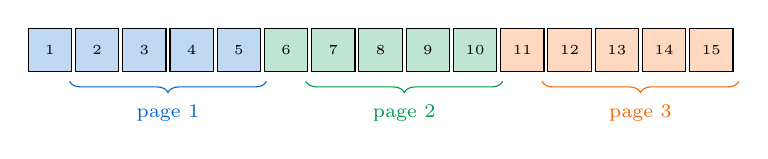
\begin{tikzpicture}[
  cell/.style={draw, minimum width=0.55cm, minimum height=0.55cm, font=\tiny},
]
  \foreach \i in {1,...,5}  { \node[cell, fill=mlblue!25]   at (\i*0.6,0) {\i}; }
  \foreach \i in {6,...,10} { \node[cell, fill=mlgreen!25]  at (\i*0.6,0) {\i}; }
  \foreach \i in {11,...,15}{ \node[cell, fill=mlorange!25] at (\i*0.6,0) {\i}; }
  \draw[decorate, decoration={brace, amplitude=4pt, mirror}, mlblue] (0.85,-0.4) -- (3.35,-0.4) node[midway, below=5pt, font=\scriptsize] {page 1};
  \draw[decorate, decoration={brace, amplitude=4pt, mirror}, mlgreen] (3.85,-0.4) -- (6.35,-0.4) node[midway, below=5pt, font=\scriptsize] {page 2};
  \draw[decorate, decoration={brace, amplitude=4pt, mirror}, mlorange] (6.85,-0.4) -- (9.35,-0.4) node[midway, below=5pt, font=\scriptsize] {page 3};
\end{tikzpicture}
\end{center}
\vspace{0.2cm}
\begin{columns}[T]
\begin{column}{0.48\textwidth}
\textbf{Request}\\
\texttt{GET /v1/predictions?page=2\&limit=5}
\end{column}
\begin{column}{0.48\textwidth}
\textbf{Response envelope}
\begin{lstlisting}[numbers=none]
{
  "items": [ ... 5 records ... ],
  "page": 2, "limit": 5, "total": 15
}
\end{lstlisting}
\end{column}
\end{columns}
\end{frame}

\begin{frame}[fragile]{Easy sample: pagination in FastAPI}
\begin{lstlisting}
HISTORY = [{"id": i, "price": 300000 + i * 1000} for i in range(1, 16)]

@app.get("/v1/predictions")
def list_predictions(page: int = 1, limit: int = 5):
    start = (page - 1) * limit
    items = HISTORY[start : start + limit]
    return {"items": items, "page": page,
            "limit": limit, "total": len(HISTORY)}
\end{lstlisting}
\end{frame}

\begin{frame}{Versioning: change without breaking clients}
\begin{columns}[T]
\begin{column}{0.5\textwidth}
\begin{center}
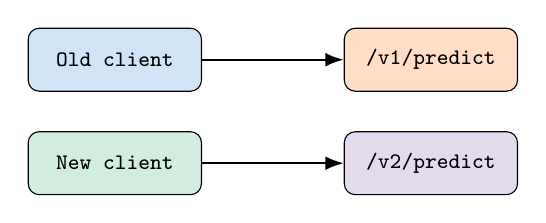
\begin{tikzpicture}[
  box/.style={draw, rounded corners, minimum width=2.2cm, minimum height=0.8cm, font=\footnotesize\ttfamily},
  arr/.style={-{Latex}, thick}
]
  \node[box, fill=mlblue!18] (c1) {Old client};
  \node[box, fill=mlgreen!18, below=0.5cm of c1] (c2) {New client};
  \node[box, fill=mlorange!22, right=1.8cm of c1] (v1) {/v1/predict};
  \node[box, fill=mlpurple!18, right=1.8cm of c2] (v2) {/v2/predict};
  \draw[arr] (c1) -- (v1);
  \draw[arr] (c2) -- (v2);
\end{tikzpicture}
\end{center}
\end{column}
\begin{column}{0.46\textwidth}
\begin{itemize}
\item Put the version in the path: \texttt{/v1}, \texttt{/v2}.
\item Adding optional fields is safe; renaming or removing is \alert{breaking}.
\item Keep \texttt{v1} alive while clients migrate.
\end{itemize}
\end{column}
\end{columns}
\end{frame}

\section{Checklist}

\begin{frame}{Good vs.\ poor API design}
\begin{center}
\begin{tabular}{p{3.6cm}p{4.2cm}p{4.2cm}}
\toprule
\textbf{Aspect} & \textbf{Poor} & \textbf{Good} \\
\midrule
\rowcolor{mlblue!8}  Naming & \texttt{/getModelData} & \texttt{GET /models/7} \\
Errors & Plain text, random codes & Uniform JSON + status code \\
\rowcolor{mlblue!8}  Lists & Returns all rows & Paginated with \texttt{total} \\
Changes & Edits live endpoint & New \texttt{/v2} version \\
\rowcolor{mlblue!8}  Fields & \texttt{SqFt}, \texttt{bed\_Rooms} & Consistent \texttt{snake\_case} \\
\bottomrule
\end{tabular}
\end{center}
\end{frame}

\section{Takeaways}

\begin{frame}{Takeaways}
\begin{enumerate}
\item An API is a contract: keep it \textbf{predictable and consistent}.
\item Name resources with \textbf{plural nouns}; let the HTTP method be the verb.
\item Define schemas (Pydantic) so inputs and outputs never surprise anyone.
\item Return the \textbf{right status code} with one standard error shape.
\item \textbf{Paginate} lists and \textbf{version} the API to avoid breaking clients.
\item Next topic: \textbf{FastAPI (Python Web Framework)}.
\end{enumerate}
\end{frame}

\end{document}
